\documentclass[10pt]{article}
\usepackage{itcep, stmaryrd, tikz, pgflibraryplotmarks, multicol}
\usepackage[margin=1in, nohead, pdftex, includefoot]{geometry}
\usepackage{MnSymbol,wasysym}
\usepackage{hyperref}


\topmargin -0.2in
\pagestyle{empty}
\singlespacing
\let\oldhat\hat
\renewcommand{\vec}[1]{\mathbf{#1}}
\renewcommand{\hat}[1]{\oldhat{\mathbf{#1}}}

\definecolor{light-gray}{gray}{0.95}
\newcommand{\code}[1]{\colorbox{light-gray}{\texttt{#1}}}

\newcommand{\headerclass}{Machine Learning Camp}
\newcommand{\headersection}{Day 2: Exploring Data with Algorithms}
\newcommand{\headertitle}{Classification using Decision Trees}

\def\C{\mathbb{C}}
\def\R{\mathbb{R}}
\parindent 0ex

%\cfoot{Kaisa Taipale, 2018}

\begin{document}
%==================================================================================================================================================
\headerclass\xspace \hspace{\stretch{1}} \headersection\\
\begin{center}{ \large \textbf{\headertitle} }\end{center}
%==================================================================================================================================================



Decision trees are another way of classifying! The cool thing about decision trees is that you can use it for many types of problems, including ones with continuous variables (like our points $(x,y)$, or height, or time, or price) and problems with categorical variables (categories like yes/no, buy/hold/sell, fitted/loose, etc). 
	Decision trees usually involved drawing out a tree, and at each branch you make a decision. When you play the game ``Twenty Questions'' you are using a decision tree.
\bigskip
\begin{center}
Big idea: Pick the right questions to separate the groups
\end{center}
\bigskip
Fake data first:
	Here is some fake data, designed to be nice. Can you ask a question about one variable (just the $x$ coordinate, or just the $y$ coordinate) that would allow you to decide if you should have a black dot or a white dot?

 
\begin{center}
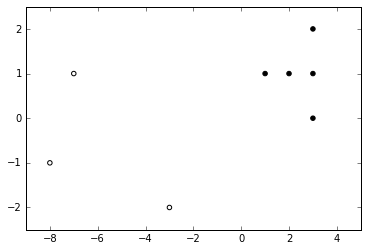
\includegraphics{TwoClusters.png}
\end{center}

Talk with your neighbor -- do you agree?


\pagebreak

Go backward this time: I'll give you a decision tree, and you draw a set of points that agrees with the decision tree rules.
\begin{center}
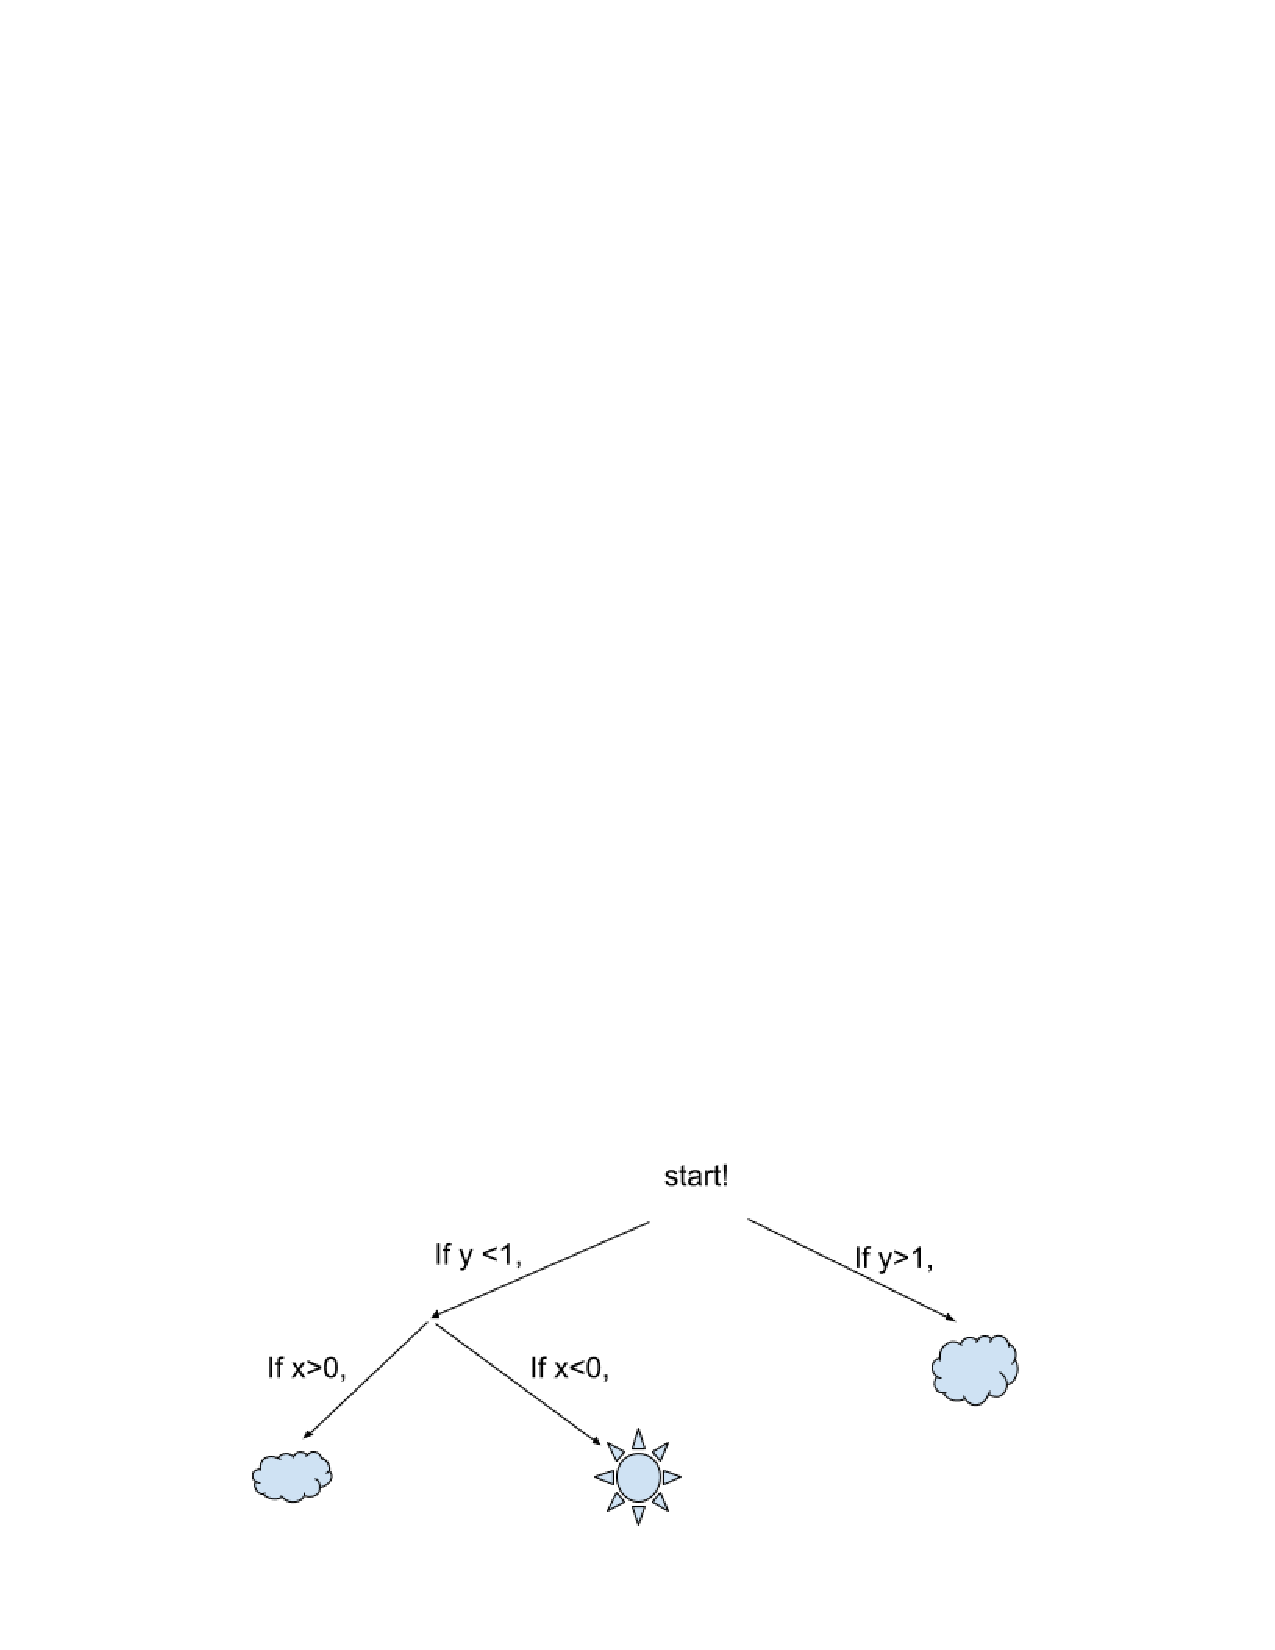
\includegraphics{SunMoonDT.pdf}
\end{center}

Draw the set of points $(x,y)$ that should be sunny and the set of points that should be cloudy according to this decision tree:
\vfill

\pagebreak


The sun and cloud symbols above are fun but also point to a set of examples people have used in textbooks about machine learning and data mining (this also means learning from data). Here's a version of this classic example:
\begin{itemize}
\item[] You are trying to figure out if your little sister's soccer game will happen today. Last year, you know the following happened:
\end{itemize}

\begin{center}

\begin{tabular}{|c|c|c|c|}
\hline
Temperature &
Rain &
Humidity &
Play \\
\hline
90 &
no &
high &
no \\
73&
no&
low&
yes \\
81&
yes&
high&
no \\
67&
no&
high&
yes\\
72&
yes&
high&
yes\\
77&
no&
low&
yes\\
96 &
no&
low&
no\\
81&
yes&
high&
no\\
58&
yes&
high&
yes\\
72&
no&
medium&
yes\\
\hline
\end{tabular}
\end{center}

\begin{enumerate}
\item On Saturday, the forecast is for 90 degrees, high humidity, and no rain. Using your intuition and the data above, do you think the game will happen? 
\vspace{1cm}
\item On Sunday, the forecast is for 70 degrees, low humidity, and rain. Using your intuition and the data above, do you think the game will happen?
\vspace{1cm}
\item Based on the data above, make a decision tree that tells you if a game will happen, based on the weather.
\vfill
Compare your decision tree with your neighbor. How can you tell if one decision tree is better or worse than another?

\pagebreak

\item Looking at the soccer game data, what do you think is the most important factor in determining whether or not a game occurs?
\vspace{1cm}

\item How does your answer to 4 affect how you would construct your decision tree?
\vfill

\item Can you think of a way to use the data to show mathematically that your answer to 4 is correct?
\vfill



\end{enumerate}


\end{document}
